%
% LaTeX report template 
%

% This is a comment: in LaTeX everything that in a line comes
% after a "%" symbol is treated as comment

\documentclass[11pt, a4paper]{article}
\usepackage{graphicx}
\usepackage{amsmath}
\usepackage{listings}
\usepackage{color}

\definecolor{dkgreen}{rgb}{0,0.6,0}
\definecolor{gray}{rgb}{0.5,0.5,0.5}
\definecolor{mauve}{rgb}{0.58,0,0.82}

\lstset{frame=tb,
  language=Python,
  aboveskip=3mm,
  belowskip=3mm,
  showstringspaces=false,
  columns=flexible,
  basicstyle={\small\ttfamily},
  numbers=none,
  numberstyle=\tiny\color{gray},
  keywordstyle=\color{blue},
  commentstyle=\color{dkgreen},
  stringstyle=\color{mauve},
  breaklines=true,
  breakatwhitespace=true,
  tabsize=3
}

\title{EE2703 Applied Programming Lab \\ Assignment 3}
\author{
  \textbf{Name}: Neham Hitesh Jain\\
  \textbf{Roll Number}: EE19B084
}\date{\today}
\begin{document}		
		
\maketitle % Insert the title, author and date

\par In this Assignment, we study the effects of Gaussian Noise (with different $\sigma$) applied to the Bessel Function on the fitting process. We plot different graphs and analyse the relationship between error in estimations of coefficients with change in $\sigma$ \\
 The major objectives for this assignment are as follows:

\begin{itemize}
\item Analysing data to extract information
\item Using least squares fitting to model the data 
\item Studying the effect of noise on the fitting process
\item Plotting graphs
\end{itemize}

\section{Introduction}

We generate a file named fitting.dat with 10 columns. The first column is the time while the remaining columns are data with a different noise amounts\\
The noise is assumed to be sampled from a normal distribution with mean 0 while the standard deviation is varied. \\

\noindent
The functions used are a linear combination of Bessel Function of the first kind and time.\\

\noindent
If n(t) is the noise function with a given $\sigma$:\\
\begin{equation*}
f(t) = A*J_{2}(t) + B*t + n(t)
\end{equation*}
\\
where A = 1.05 and B = -0.105 are constants.\\~\\


\noindent
The Probability Distribution Function of noise is given by

 \begin{equation*}
Pr(n(t)|\sigma) = \frac{1}{\sigma\sqrt{2\pi}}exp(\frac{-n(t)^2}{2\sigma^2})
\end{equation*}
\\where $\sigma$ is given by 
\begin{verbatim}
    variance = logspace(-1,-3,9)
\end{verbatim}
and thus noise is assumed to be normally distributed.\\


\section{Objectives}
\subsection{Generation and Loading of Data}
\par The data is generated using the code generate\_data.py. It computes all the values of the sample function with 9 different values of standard deviation.The data is stored in a .dat file.The first column represents time values and the rest of the columns represent the function value with different amount of noise added. We import the .dat file in our program using loadtxt function of NumPy library\\

\subsection{Plotting the data}
\par We plot the all the data points with varying noise alongside the true value using pyplot.

\begin{lstlisting}

#Helper Function for Question 3 and 4
def plot_fitting_cols(time,vals,ground_truths,scl):
    vals=c_[vals,ground_truths]
    figure(0)
    plot(time,vals)
    xlabel(r"Time $\rightarrow$")
    ylabel(r"$f(t)+Noise \rightarrow$")
    title("Plotting fitting.dat and ground truth values")
    scl=[f"Standard Deviation={round(i,4)}" for i in scl]
    legend(list(scl)+["True Value"])
    grid(True)
    #show()
    savefig("plots/Ques3_4.jpg")
    close()
    
\end{lstlisting}


\begin{figure}[!tbh]
   	\centering
   	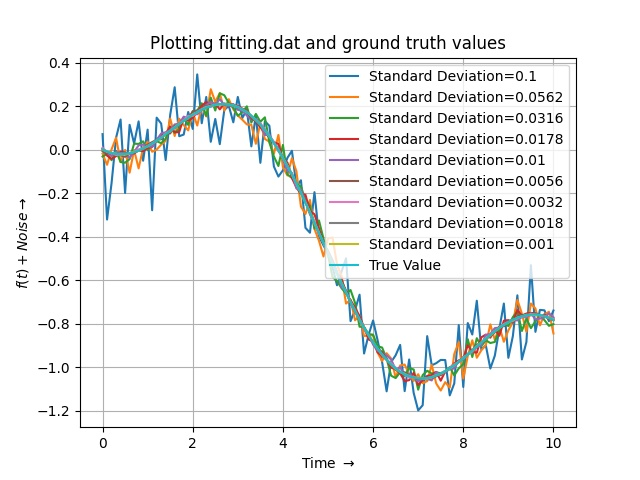
\includegraphics[scale=0.7]{plots/Ques3_4.jpg}  % Mention the image name within the curly braces. Image should be in the same folder as the tex file. 
   	\caption{Plotting the columns of fitting.dat and ground truth function}
   	\label{fig:Data plot}
   \end{figure} 

\subsection{Error plots}
We visualise the error in the measurement using the \textit{errorbar()} function.
The graph has been obtained by plotting the first column in the data file which corresponds to $sigam = 0.1$\\
The true value has also been plotted for reference.

\begin{lstlisting}

#Helper function for plotting the error bars
def plot_errorbars(time,values,ground_truth):
    figure(1)
    std_dev = std(values[:,0]-ground_truth)
    xlabel(r"Time $\rightarrow$")
    ylabel(r"f(t) $\rightarrow$")
    title(f"Data Points for stddev={round(std_dev,3)} along with exact function")
    errorbar(time[::5],values[:,0][::5],std_dev,fmt='ro')
    plot(time,ground_truth)
    legend(["f(t)","Error Bar"])
    #show()
    savefig("plots/Ques5.jpg")
    close()

\end{lstlisting}

\begin{figure}[!tbh]
   	\centering
   	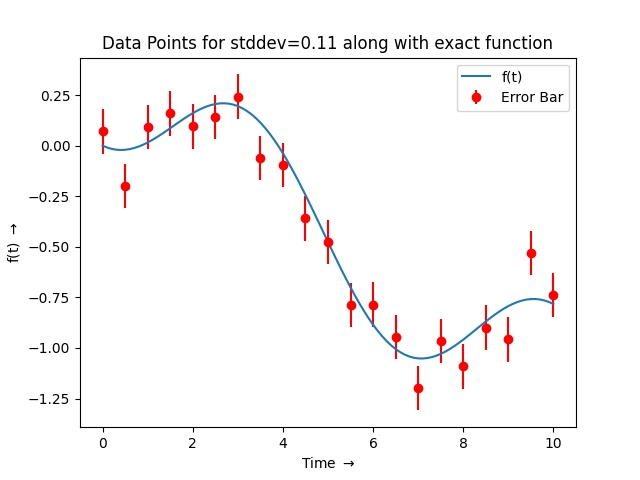
\includegraphics[scale=0.6]{plots/Ques5.jpg}  % Mention the image name within the curly braces. Image should be in the same folder as the tex file. 
   	\caption{Error bars for $\sigma$ = 0.1 along with exact function}
   	\label{fig:Error bar}
   \end{figure}
   

\subsection{Generating Matrix}
\par We transform this problem into a matrix multiplication as it becomes faster for computing 
%\begin{equation}

\begin{center}
     $   g(t,A,B) = 
    \begin{pmatrix}
    J_{2}(t_{1})& t_{1}\\
    J_{2}(t_{2}) & t_{1}\\
    ... & ...\\
    J_{2}(t_{n})& t_{n}
    \end{pmatrix}
     \begin{pmatrix}
        A \\
        B
    \end{pmatrix} = M\cdot p$
    
\end{center}
\par We generate the  M matrix and check if the true values satisfies the Ao and Bo value. Since the MSE error that we get is 0, we can say that the 2 vectors are equal.
\begin{lstlisting}
#Function for constructing the M matrix
def construct_M(time):
    return c_[sp.jn(2,time),time]

#Function calls in main
M = generate_M(x_matrix)
M=construct_M(time_values)
AB=np.array([1.05,-0.105])
#Confirms whether M*AB and the function g(t,A,B) are equal or not
print("The mean squared error between M*AB and g(t,A,B) is: ",calculate_mse(matmul(M,AB),g(time_values,1.05,-0.105)))

\end{lstlisting}
%\end{equation}
    

\subsection{Generating Error Matrix and plotting the Contour Plots}
We know that the true values satisfies the equation of the form:\\
\begin{equation*}
g(t,A,B) = AJ_{2}(t)+Bt 
\end{equation*}
Our aim is to find appropriate vales of A and B so that given data best fits into the equation.\\\\Thus we vary our values of A and B within the given range and generate an epsilon matrix ($\epsilon_{ij}$) between the data (1st column in our case) and the assumed model. 
\begin{equation}
    \epsilon_{ij} =  \frac{1}{101}\sum_{k=0}^{101}(f(x)-g(t_k,A_i,B_j))^2
\end{equation} \\
After generating such a matrix we plot the contour plot of such an epsilon matrix. \\
\begin{lstlisting}
def plot_contours(values,time):
    figure(2)
    A_range=arange(0,2.1,0.1)
    B_range=arange(-0.2,0.01,0.01)
    epsilon_matrix = zeros((len(A_range),len(B_range)))
    for count_A,A in enumerate(A_range):
        for count_B,B in enumerate(B_range):
            epsilon_matrix[count_A][count_B] = calculate_mse(values[:,0],g(time,A,B))
    contour_obj = contour(A_range,B_range,epsilon_matrix,levels=arange(0,20*0.025,0.025),cmap="magma")
    clabel(contour_obj,contour_obj.levels[0:5],inline=True,fontsize=10)
    title('Contour Plot of Error')
    xlabel(r'A $\rightarrow$',size=12)
    ylabel(r'B $\rightarrow$',size=12)
    plot(1.05, -0.105,'ro', label = 'Exact Value')
    annotate("Exact Value",xy = [0.8,-0.100])
    savefig("plots/Ques8.jpg")
    close()

\end{lstlisting}


\noindent
\\
From the below plot we can clearly see that there exist a single minimum.
\\
\begin{figure}[!tbh]
   	\centering
   	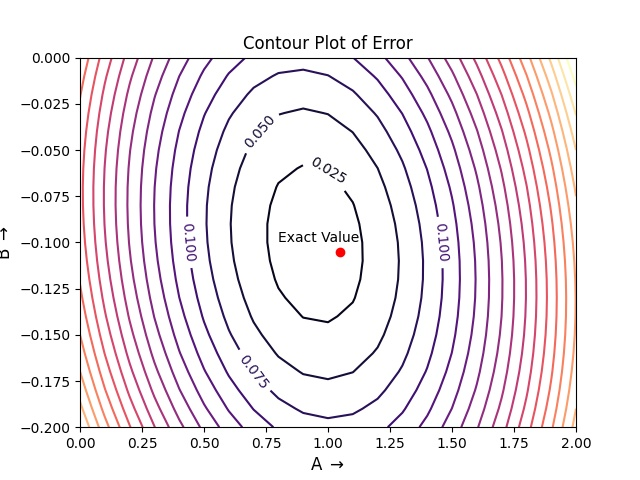
\includegraphics[scale=0.7]{plots/Ques8.jpg}  % Mention the image name within the curly braces. Image should be in the same folder as the tex file. 
   	\caption{contour plot for $\epsilon_{ij}$ }
   	\label{fig:Contour plot}
   \end{figure}
\\
\newpage
\subsection{Finding the values of parameters A and B}
\par Now, we can estimate the values of A and B by minimizing $|M*(AB)-C|$ where C is one of the columns of data. We can do this using the \emph{scipy.linalg.lstsq()} function.\\~\\
Thus, we find the values of A and B and store it in a NumPy array.

\subsection{Error plots for different scales}
\par For the above calculated A and B, we find the absolute error between the calculated and the true values and plot them in linear and log scale both.



\subsubsection{Linear scale}
We plot the graph of error with varying noise parameters
\begin{lstlisting}

#Helper function for plotting the contour plot
def plot_variation_of_error(scl,error_a,error_b):
    figure(3)
    plot(scl,error_a,'r--')
    scatter(scl,error_a)
    plot(scl,error_b, 'b--')
    scatter(scl,error_b)
    legend(["Aerr","Berr"])
    title("Variation Of Error with Noise")
    xlabel(r'$\sigma_{n}\rightarrow$',size=10)
    ylabel(r'Absolute Error $\rightarrow$',size=10)
    savefig("plots/Ques10.jpg")
    close()

\end{lstlisting}


\noindent
\\   
\textbf{The errors in the estimation of A and B are non-linear with respect to $\sigma_{n}$}

\begin{figure}
   	\centering
   	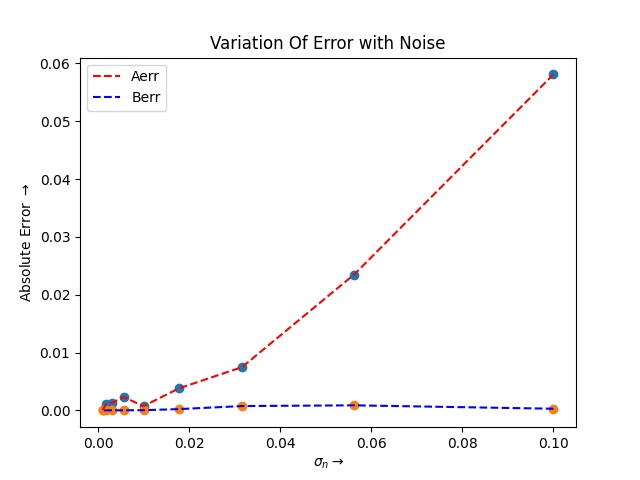
\includegraphics[scale=0.6]{plots/Ques10.jpg}  % Mention the image name within the curly braces. Image should be in the same folder as the tex file. 
   	\caption{A and B error in linear scale}
   	\label{fig:A and B err in linear scale}
\end{figure}

\subsubsection{Loglog scale}
Now we plot the graph in log scale
\begin{lstlisting}
def plot_log_variation_of_error(scl,error_a,error_b):
    figure(5)
    stem(scl,error_a,'ro')
    loglog(scl,error_a,'ro')
    loglog(scl,error_b,'bo')
    stem(scl,(error_b),'bo')
    xlabel(r'$\sigma_{n}\rightarrow$',fontsize=15)
    ylabel(r'Error$\rightarrow$',fontsize=15)   
    legend(["Aerr","Berr"])
    title("Stem plot showing variation of error with standard deviation")
    savefig("plots/Ques11.jpg")
    close()
    
\end{lstlisting}

\begin{figure}
   	\centering
 
   	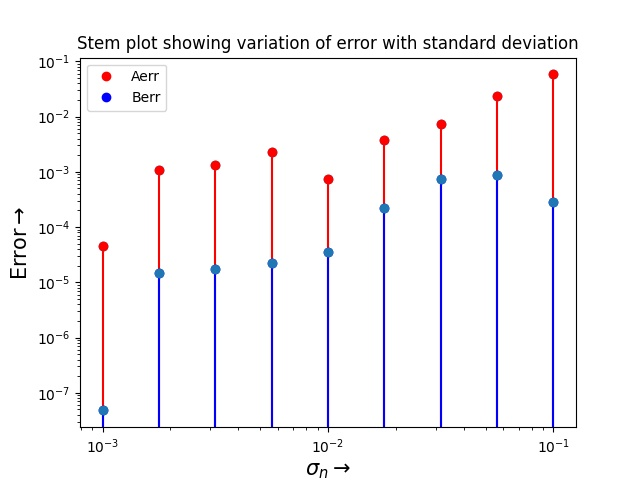
\includegraphics[scale=0.6]{plots/Ques11.jpg}  % Mention the image name within the curly braces. Image should be in the same folder as the tex file. 
   	\caption{A and B error in log scale}
   	\label{fig:A and B err in log scale}
\end{figure}
  
\section{Conclusions}
For the given noisy function the best possible estimates for A and B were
obtained by minimizing the mean squared error with the true value.It is
observed that error in estimation of the model parameters changes approximately linearly with respect to $\sigma$ in the log scale

 
\end{document}